\begin{appendices}

\chapter{UML Activities Tutorial}
\label{appx:tutorial}
The following pages contain the complete document for the Reactive Blocks \gls{uml} Activities tutorial described in Ch.~\ref{ch:reactive_blocks_tutorial}.
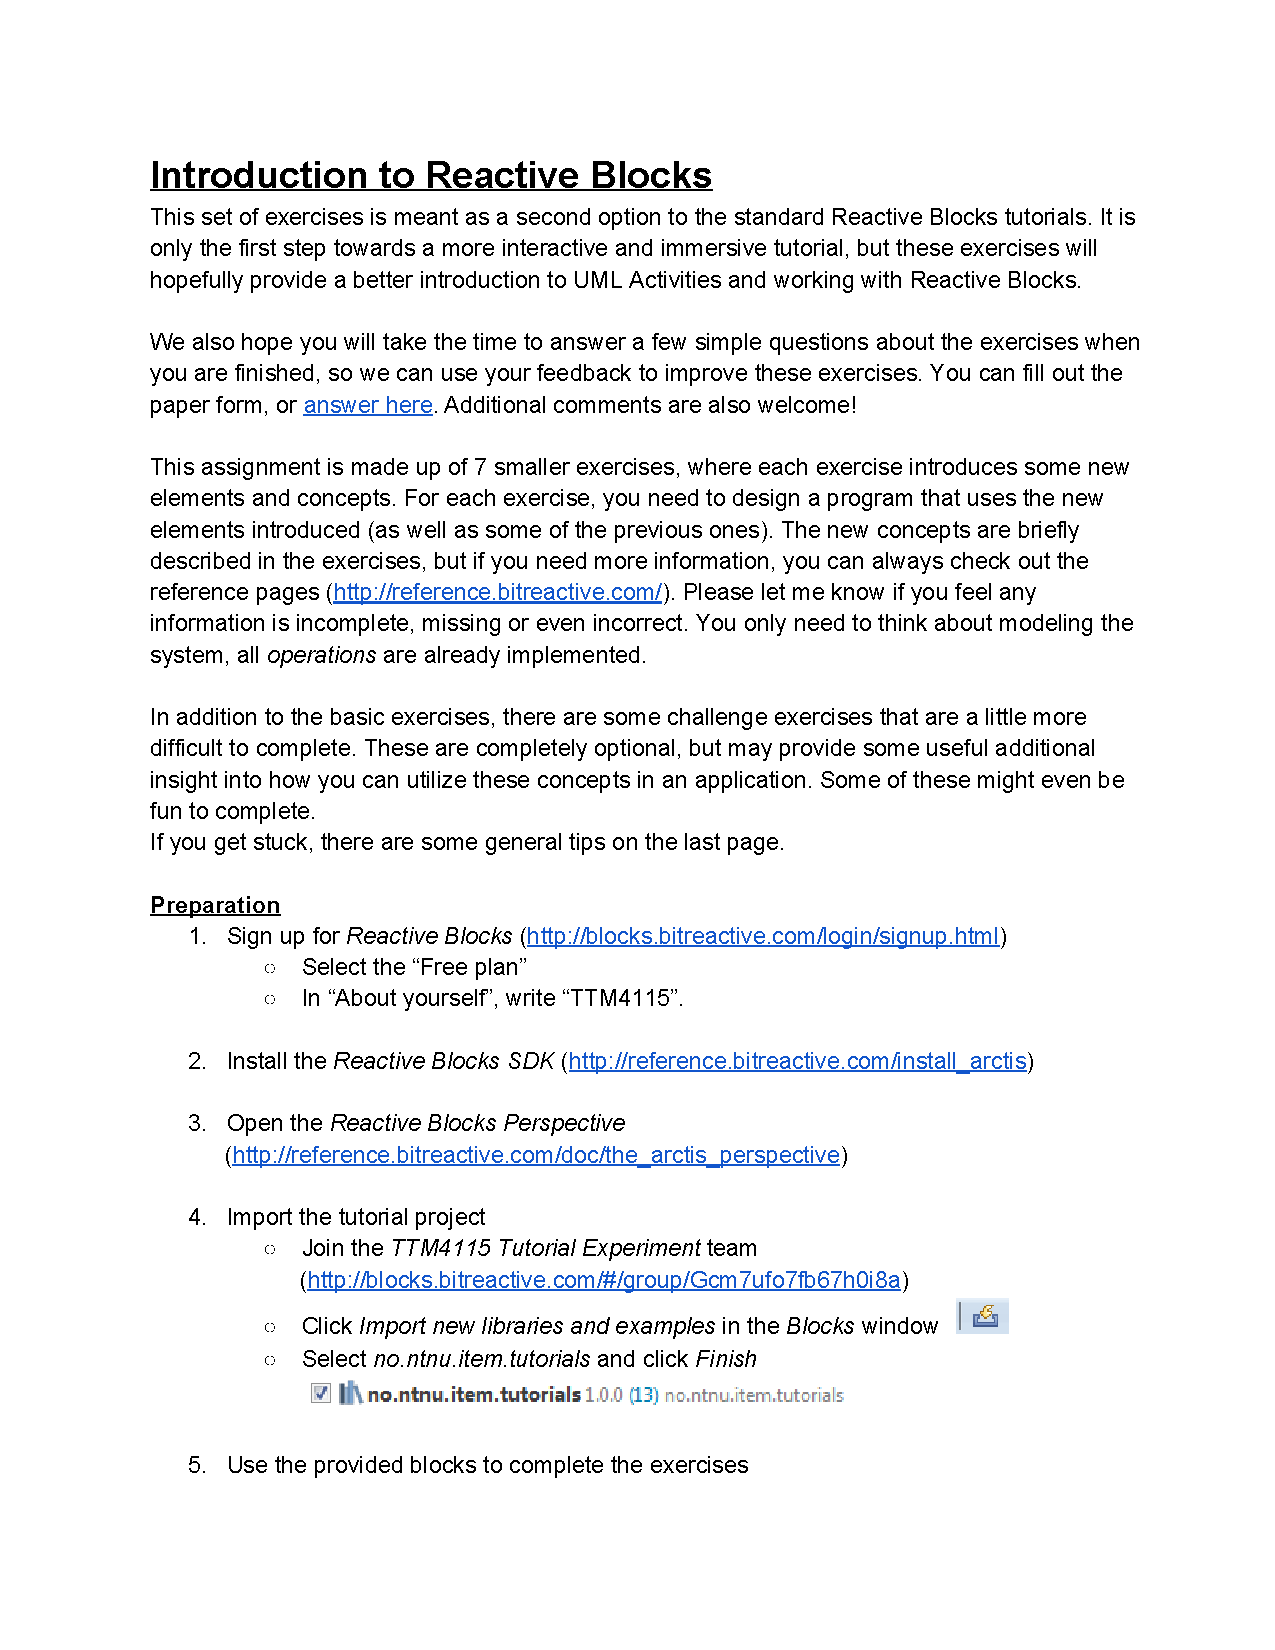
\includepdf[pages={-}]{tutorial_exercises.pdf}

\chapter{Tutorial Feedback Form}
\label{appx:feedback_form}

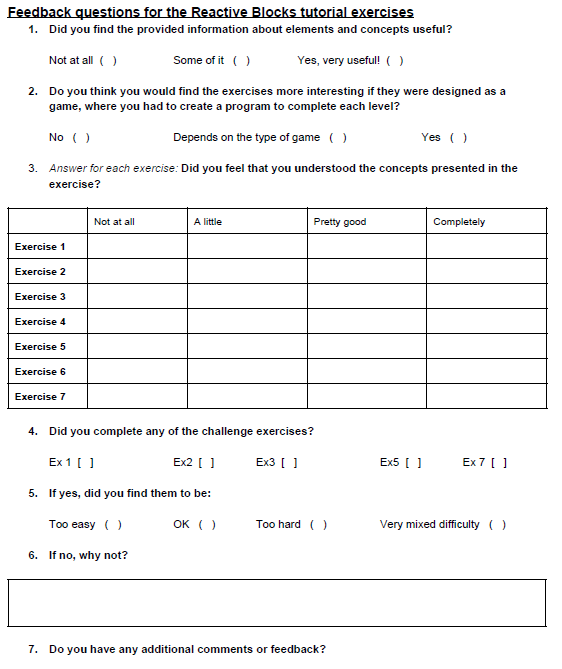
\includegraphics[scale=0.75]{tutorial_feedback}

\chapter{Tutorial User Test Data}
\label{appx:tutorial_test_data}
This section contains all the data gathered with the feedback forms (Appx.~\ref{appx:feedback_form}) in the user test for the Reactive Blocks/\gls{uml} Activities tutorial (Ch.~\ref{ch:reactive_blocks_tutorial}).

\begin{figure}[htp]
	\centering
	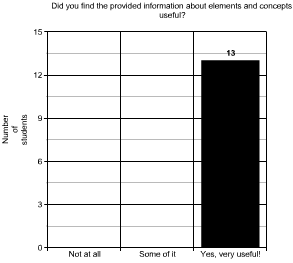
\includegraphics[scale=0.80]{feedback_form_q1}
	\caption[Results from feedback form question 1]{Results from question 1 of the feedback form (Appx.~\ref{appx:feedback_form}). The total number of students was 13.}
	\label{fig:feedback_form_q1}
\end{figure}

\begin{figure}[htp]
	\centering
	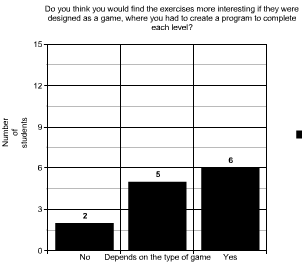
\includegraphics[scale=0.80]{feedback_form_q2}
	\caption[Results from feedback form question 2]{Results from question 2 of the feedback form (Appx.~\ref{appx:feedback_form}). The total number of students was 13.}
	\label{fig:feedback_form_q2}
\end{figure}

\begin{figure}[htp]
	\centering
	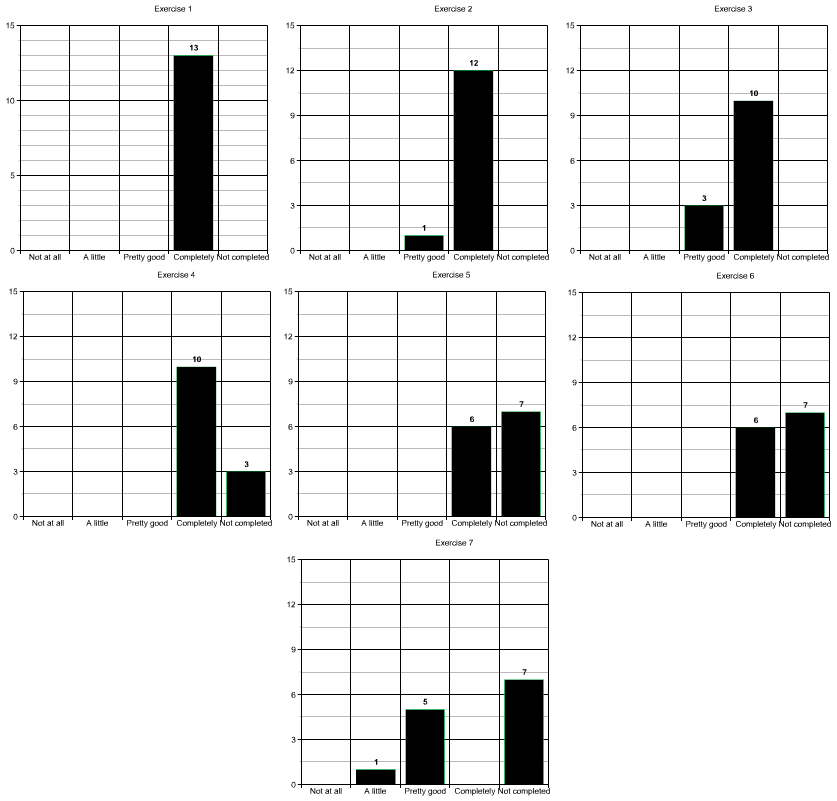
\includegraphics[scale=0.55]{feedback_form_q3}
	\caption[Results from feedback form question 3]{Results per exercise from question 3 of the feedback form (Appx.~\ref{appx:feedback_form}). The value on the y-axis for all graphs is the number of students who chose that answer. The total number of students was 13.}
	\label{fig:feedback_form_q3}
\end{figure}

\begin{figure}[htp]
	\centering
	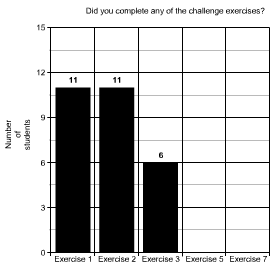
\includegraphics[scale=0.80]{feedback_form_q4}
	\caption[Results from feedback form question 4]{Results from question 4 of the feedback form (Appx.~\ref{appx:feedback_form}). The total number of students was 13.}
	\label{fig:feedback_form_q4}
\end{figure}

\begin{figure}[htp]
	\centering
	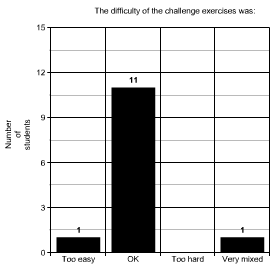
\includegraphics[scale=0.80]{feedback_form_q5}
	\caption[Results from feedback form question 5]{Results from question 5 of the feedback form (Appx.~\ref{appx:feedback_form}). The total number of students was 13.}
	\label{fig:feedback_form_q5}
\end{figure}

\chapter{Feedback Form for the Game Usability Test}
\label{appx:game_feedback_form}

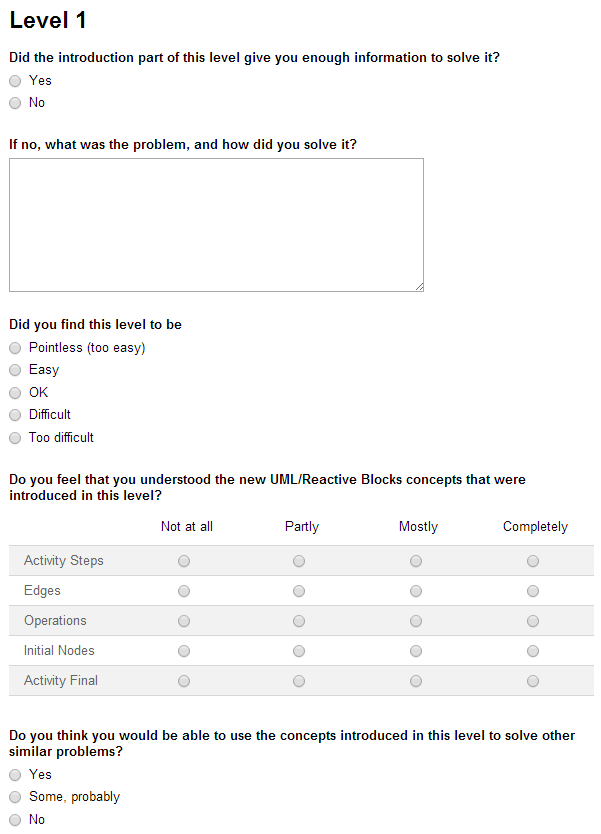
\includegraphics[scale=0.60]{usability_quiz}







\end{appendices}